\NeedsTeXFormat{LaTeX2e}
\documentclass[11pt]{article}
\usepackage[utf8]{inputenc}
\usepackage[T1]{fontenc}
\usepackage{ae}
\usepackage[intlimits, sumlimits, namelimits]{amsmath}
\usepackage{bbm}
\newcommand{\inp}[1]{\ensuremath{\left(#1\right)}}
\newcommand{\sqr}{\ensuremath{^{2}}}
\newcommand{\cube}{\ensuremath{^{3}}}
\newcommand{\set}[1]{\ensuremath{\mathbbm{#1}}}
\newcommand{\norm}[1]{\ensuremath{\left|#1\right|}}
\newcommand{\svec}[3]{\ensuremath{\inp{\hspace{-.8ex}\begin{array}{r}#1\\#2\\#3\end{array}\hspace{-.4ex}}}}
\newcommand{\entspr}{\ensuremath{\,\,\hat{=}\,\,}}%
\newcommand{\dx}[1][x]{\ensuremath{\textnormal d #1}}
\newcommand{\trace}{\textnormal{Tr}}

% For stupid thinkos:
\newcommand{\cross}{\times}
\newcommand{\dell}{\partial}

\usepackage{array}
\setlength{\extrarowheight}{.2mm}
\usepackage{hyperref}
\usepackage{graphics,graphicx,fancyvrb}
%Raender einstellen
%\usepackage[a4paper, margin=15mm, top=30mm]{geometry}
\usepackage[a4paper]{geometry}
\usepackage{lastpage}
\usepackage{fancyhdr}
	\lhead{Moritz Lenz}
	\chead{\bfseries{-- \thepage\ --}}
	\rhead{\thetitle}
	\lfoot{}
	\rfoot{}
	\cfoot{}
	\pagestyle{fancy}
\pagestyle{empty}

\sffamily

\bibliographystyle{alpha}


\author{Moritz Lenz}
\title{Theory}
\begin{document}
\maketitle

Consider a two-dimensional conductor of width $W$ and length $L$. If these two
dimensions  are large enough, the conductance is

\begin{align}
    G = \sigma \frac{W}{L}
\end{align}

where $\sigma$ is a material specific parameter, and independent of the
geometry of the conductor. \emph{Large enough} means in this context
specifically that both lengths are large compared to all of three
characteristic lengths: the Fermi wavelength, the mean free path and the
phase-relaxation length.

The mean free path is the average distance which a charge carrier can travel
before it is scattered (by an impurity, electrons or phonons), and thus loses
momentum.

If the length of the conductor is smaller than the mean free path, most
electrons travel through it without scattering, and one could naively assume
that this means the resistance is zero.

Still experiments show that a finite resistance can be observed. That's
because the sample can't be measured in isolation; it is attached to the
macroscopic measuring system through \emph{leads}. Even if the leads are very
good conductors themselves, a contact resistance arises. So the theory has to
take into account both the sample and the leads.

The following explanations are mostly taken from \cite{datta}.

\subsection*{Landauer Formula}

\begin{figure}
    \begin{center}
        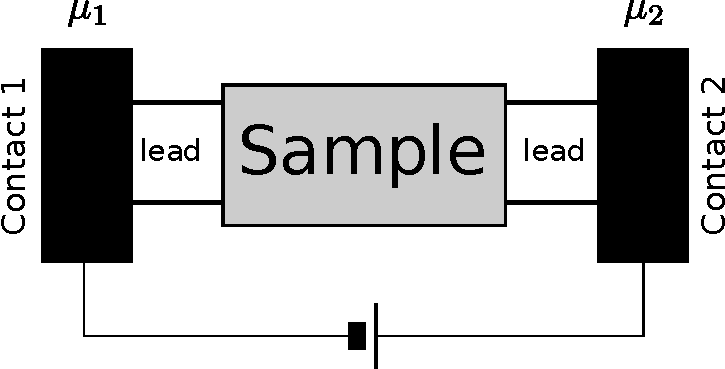
\includegraphics[width=0.5\textwidth]{sample-leads}
    \end{center}
    \caption{Schematic setup to derive the Landauer Formula}
    \label{fig:sample-leads}
\end{figure}

The sample is attached to two leads, which we assume to be perfect, ballistic
conductors with $M$ modes each. We assume that the contacts are
reflectionless, that is electrons can travel from the sample into the contacts
without reflection.

This means that the $k_x$ states in the left lead are occupied by electrons
coming from contact 1, and thus have the same electrochemical potential as
the contact, $\mu_1$. Likewise the $-k_x$ states in the right lead have the
potential $\mu_2$.

At zero temperature, only electrons with energies between $\mu_1$ and $\mu_2$
are transported, and the influx from the left lead is
$I_1^+ = (2e/h)M(\mu_1-\mu_2)$. We call the transmission probability through
the sample $T$, so the outflux from lead 2 is $I_2^+ = T I_1^+$, the rest
is reflected back: $I_1^- = (1-T) I_1^+$. The net current $I$ then is

\begin{align}
    I = I_1^+ - I_1^- = \frac{2e}{h} M T (\mu_1 - \mu_2)
\end{align}

The conductance is

\begin{align}
    G = \frac{I |e|}{\mu_1 - \mu_2} = \frac{2 e^2}{h} MT
\end{align}

\subsection*{Transmission and Green's functions}

To calculate the value $T$, one can make use of the so-called \emph{Green's
functions}. A Green function $G$ is, loosely speaking, an inverse of a
differential operator $D$. More precisely if the relation between an
excitation $\delta$ and a response $R$ is $D R = \delta$, then every
operator $G$ for
which the equation $R = G \delta$ holds is called a Green's function.

To calculate the wave function $\psi$ in response to an excitation $\delta$ at a
given energy $E$ we can use the inhomogeneous Schrödinger Equation

\begin{align}
    \label{eq:green-define}
    (E - H) \psi = \delta
\end{align}

Where $H$ is the Hamiltonian operator. In a one-dimensional wire oriented
along the $x$ axis we expect an excitation of the form
$\delta = \delta(x - x_0)$ to result in two waves propagating away from $x_0$,
so our ansatz is

TODO: explicit form of $H$

\begin{align}
    G(x, x_0) = \begin{cases}
        A^+ e^{i k(x-x_0) } \qquad \textnormal{ for } x > x_0 \\
        A^- e^{-i k(x-x_0) } \qquad \textnormal{ for } x < x_0 \\
    \end{cases}
%    \left\{   \right.
\end{align}

This function satisfies Eqn. \ref{eq:green-define} for every point $x \not=
x_0$  for $ k = \sqrt{\frac{2mE}{\hbar^2}}$.

From the boundary conditions

\begin{align}
    G(x = x_0 + 0, x_0) - G(x = x_0 - 0, x_0) &= 0 \\
    \frac{\partial G(x, x_0)}{\partial x}\left.\right|_{x=x_0 +0}
    -\frac{\partial G(x, x_0)}{\partial x}\left.\right|_{x=x_0 -0}
        &= \frac{2m}{\hbar^2}
\end{align}

we obtain $A^+ = A^- = -\frac{i}{\hbar v}$ where $v := \frac{\hbar k}{m} $.

We call this particular solution the \emph{retarded Green's function} $G^R$,
to distinguish it from a second solution with opposite sign both in the $A$s
and in the exponent, which we call the \emph{advanced} Green's function $G^A$.

In a wire with finite width multiple modes can propagate, but since we can
separate the $x$ and $y$ components, the Green's functions become only
marginally more complex:

\begin{align}
    G^R(x, x_0) = \sum_m A^\pm_m \chi_m(y) e^{i k_m |x - x_0|}
\end{align}

where the transverse wave functions $\chi_m(y)$ satisfy the Schrödinger
Equation in $y$ direction with eigenvalue $\epsilon_m$.

Orthogonality of the different $\chi_m(y)$ functions and boundary conditions
give us an expression for the amplitudes:

\begin{align}
    A^\pm = - \frac{i}{\hbar v_m} \chi_m(y_0)
\end{align}

If $E$ is an eigenvalue of $H$, $(E-H)^{-1}$ might not exist. One guards
against potential singularities by introducing a small number $\eta$ and
defines

\begin{align}
    G^R &= \left( (E + i \eta)\mathbf{1} - H \right)^{-1}\\
    G^A &= \left( (E - i \eta)\mathbf{1} - H \right)^{-1}
\end{align}

One can (with some approximations) obtain a matrix representation for $H$
(TODO: reference) and thus calculate the inverse, as long as we don't consider
open systems.

\begin{figure}
    \begin{center}
        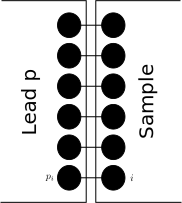
\includegraphics[height=5cm]{coupling-sample-lead}
    \end{center}
    \caption{Coupling between a lead and the sample}
    \label{fig:coupling-sample-lead}
\end{figure}

When we consider a discrete lattice both in the sample and in the leads, we
can couple adjacent lattice points in the sample and a lead as shown in Fig.
\ref{fig:coupling-sample-lead}.

The overall Green's function for both sample and lead can be partitioned into
a Green's function for the sample $G_s$, for the lead $G_p$ and two coupling
Green's functions $G_{sp}, G_{ps}$

\begin{align}
\left(
    \begin{array}{ll}
        G_p    & G_{ps}\\
        G_{sp} & G_s
    \end{array}
\right)
=
\left(
    \begin{array}{ll}
        (E + i\eta)\mathbf{1} - H_p   & \tau_p\\
        \tau_p^\dagger                & E\mathbf{1} - H_s
    \end{array}
\right)^{-1}
\label{eq:coupling-green}
\end{align}

Where $\tau_p$ is the coupling matrix for lead $p$, and contains only non-zero
entries $t$ for matrix elements connecting adjacent sites in lead and sample.

From \ref{eq:coupling-green} we can find an expression for $G_s$:

\begin{align}
    G_s = (E\mathbf1 - H_s - \tau^\dagger g_p^R \tau_p )^{-1}
\end{align}

Where $g_p^R$ is the retarded Green's function for the isolated lead $p$,

\begin{align}
    g_p^R = ((E+i\eta)\mathbf1 - H_p)^{-1}
\end{align}

$g_p^R$ can often be calculated analytically. We call the term $\tau^\dagger
g_p^R \tau_p$ \emph{self-energy}. When multiple independent leads are attached
to the same sample, the effects of the self-energies for each lead simply add
up, and we get

\begin{align}
    G_s^R &= \left(E\mathbf1 - H_s - \sum_p \Sigma^R_p\right)^{-1} \\
    \textnormal{with } \Sigma^R_p &= \tau^\dagger g_p^R \tau_p
\end{align}

It can be shown \cite{baranger} that the transmission $T_{pq}$ from lead
$q$ through the sample into lead $p$ is

\begin{align}
    T_{pq} = \trace(\Sigma_p G_s^R \Sigma_q G_s^A)
\end{align}

This allows numeric calculation of transmission coefficients for
arbitrary Hamiltonian operators, and is thus independent of the individual
phenomena we're looking at.

\subsection*{Rashba Spin-Orbit Coupling}

TODO

\subsection*{Tight Binding Hamiltonian}


In order to numerically evaluate the Green's function, we
discretize the sample into sites and assume that electrons only travel from
one site to an immediate neighbor. This allows us to represent the
Hamiltonian and other differential operators by a finite matrix.

% TODO: references
The nearest neighbor approximation is quite common in transport calculations,
and comes from the linear combination of atomic orbits (LCAO) ansatz, where
one assumes that the overlap between localized electron orbitals decreases
exponentially with distance.

In a two-dimensional square lattice the distance to the next nearest
neighbors is $\sqrt{2} a$ (where $a$ is the lattice constant), so one can
approximate that the overlap is $e^{-\sqrt{2}} \approx 0.24$. For a simulation
that tries to reproduce exact physical behavior of a sample one would have to
include the next-nearest neighbor hopping, and maybe even one further step
($e^{-2} \approx 0.14$).

But since our model is an effective one, we have to give up that claim
anyway, and instead ask ourselves if next-nearest neighbor hopping or higher
orders contribute any new physics, in terms of symmetries. To the best of our
knowledge that is not the case, so we keep the nearest neighbor approximation.

For a two-dimensional electron gas with Rashba spin-orbit coupling (of
strength $\alpha$) the Hamiltonian is

\begin{equation}
    H = \frac{1}{2 m^*} (p_x^2 + p_y^2) +
    \frac{\alpha}{\hbar} \inp{p_y\sigma_x - p_x\sigma_y}
\end{equation}

To map this to a discrete lattice we substitute the derivation by a discrete
difference, so $\dell_x f(x)|_{x_0}$ becomes $(f(x_0+a) - f(x_0))/a$. For the
second derivation we chose the symmetric difference $\dell_x^2 f(x)_{x_0} =
(f(x_0+a) - f(x_0-a))/2a$. In the continuum limit $a \mapsto 0$ both reproduce
the derivation exactly.

Written in terms of creation and destruction operators we obtain

\begin{align}
    H   &= H_0 + H_r\\
    H_0 &= \sum_{n,\sigma} \epsilon_0 c^{\dagger}_{n\sigma} c_{n\sigma}
           - \sum_{n,\delta,\sigma} t c^\dagger_{n\sigma} c_{n,\sigma} +
           \textnormal{H.c.}\\
    H_r &= \frac{-\alpha}{2 a_0} \sum_m
        -i( c^\dagger_{m,\uparrow|} c_{m+a_y,\downarrow}
            + c^\dagger_{m,\downarrow} c_{m+a_y,\uparrow})
         + c^\dagger_{m,\uparrow|} c_{m+a_x,\downarrow}
            + c^\dagger_{m,\downarrow} c_{m+a_x,\uparrow}
\end{align}

where $n$ runs over all lattice sites, $\delta$ over $\uparrow$ and
$\downarrow$, and $a_x$ and $a_y$ denote the shift to the nearest neighbor in
$x$ and $y$ direction, respectively. (Note that we assume that the lattice is
equally spaced in $x$ and $y$ direction, $+a_x$ just means "go to the next
neighbor in $x$ direction).

Assume we have a quadratic system of $N \times N$ lattice sites.
For a two-dimensional system we enumerate all lattice sites row by row, and
use the result as the index to the Hamiltonian. To incorporate spin, we
identify the indexes that were assigned so far with spin-up, and add $N^2$ to
each index to obtain the matrix index for spin-down.

For example if our system were of size $3 \times 3$, the left-most site in the
first row has index $i = 1$, and the left-most site in the second row has
index $j = N + 1 = 4$ (both spin down). The interaction term (without spin
flip) between these two sites can thus be found at $H_{i,j} = H_{1,4}$. The
interaction that involves a spin flip from $\uparrow$ to $\downarrow$ is
described by $H_{i, j+N^2} = H_{1, 13}$.

\begin{figure}
    \begin{align*}
        H &= \inp{
           \begin{array}{cc}
                H_{kin}  & H_{spin} \\
                H_{spin}^\dagger & H_{kin} \\
           \end{array}} \\
           %
        H_{kin} &= \inp{
            \begin{array}{ccccccccc}
                -4t & t &  & t\\
                t & -4t & t &  & t &  &  & 0\\
                & t & -4t & 0 &  & t\\
                t &  & 0 & -4t & t &  & t\\
                & t &  & t & -4t & t &  & t\\
                &  & t &  & t & -4t & 0 &  & t\\
                &  &  & t &  & 0 & -4t & t\\
                & 0 &  &  & t &  & t & -4t & t\\
                &  &  &  &  & t &  & t & -4t\end{array}
        } \\
        %
        H_{spin} &= \inp{
            \begin{array}{ccccccccc}
                0 & -r &  & r\\
                r & 0 & -r &  & r &  &  & 0\\
                & r & 0 & 0 &  & r\\
                -r &  & 0 & 0 & -r &  & r\\
                & -r &  & r & 0 & -r &  & r\\
                &  & -r &  & r & 0 & 0 &  & r\\
                &  &  & -r &  & 0 & 0 & -r\\
                & 0 &  &  & -r &  & r & 0 & -r\\
                &  &  &  &  & -r &  & r & 0\end{array}
        }
    \end{align*}
    \caption{Tight binding Hamiltonian for $ 3 \times 3 $ lattice sites}
    \label{fig:hamiltonian}
\end{figure}

Figure \ref{fig:hamiltonian} shows an example Hamiltonian for a system of
$3 \times 3$ lattice sites with Rashba spin-orbit coupling (and no magnetic
field).

Sites at the edge of the sample have no hopping element to a neighboring site
at the outside of the sample, so we have hard wall boundary conditions. All
interaction with the outside world is modeled through the self-energy induced
by the attached leads.


\bibliography{bib}

\end{document}

% vim: ts=4 sw=4 expandtab spell spelllang=en_us tw=78
